\documentclass[10pt]{extarticle} % Usa fonte de 10pt
\usepackage{graphicx} % Required for inserting images
\usepackage{float}
\usepackage{geometry}
\usepackage{hyperref}
\usepackage{minted}
\setminted{
  breaklines=true, % Permite quebra de linha
  breakanywhere=true, % Permite quebra em qualquer posição
  fontsize=\small % Define tamanho da fonte para ajudar com overflow
}

\geometry{margin=1in}

\title{Trabalho de Implementação 1 - Heurísticas e Metaheurísticas}
\author{Francisco Teixeira Rocha Aragão - 2021031726}


\date{Data de entrega: 21 de novembro de 2024}

\begin{document}

\maketitle

\section{Introdução}

O presente trabalho busca resolver de maneira aproximada o problema do caixeiro viajante (TSP), fazendo uso de heurísticas gulosas em sua implementação. Como o problema pertence a classe NP, faz-se necessário o uso de tais estratégias, sendo feito especificamente uma heurística gulosa no trabalho. Abaixo encontra-se mais informações sobre a implementação além dos resultados obtidos.

\section{Heurísticas utilizadas}

Primeiramente sobre a heurística utilizada, a estratégia implementada no trabalho refere-se a heurísticas construtivas, ou seja, heurísticas em que a solução é construída do zero, desde o início até a resolução do problema. Iniciando-se assim de uma solução vazia, obtendo-se uma solução parcial a cada iteração em que ao final transforma-se em uma solução completa válida.

Desse modo, a estratégia utilizada foi baseada em uma abordagem gulosa, em que a cada ponto (ou cidade), o próximo trajeto escolhido é aquele com a menor distância. Desse modo, inicia-se a partir de uma cidade (será explicado mais frente), e a cada iteração novas cidades são adicionadas no caminho até todas as cidades serem visitadas, voltando assim ao vértice inicial resolvendo o problema. Com isso, garante-se a validade da solução retornada, em que a cada iteração acrescenta-se uma nova cidade não visitada anteriormente, terminando o algoritmo até visitar a última cidade, retornando ao ponto inicial.

Sobre o ponto inicial escolhido, duas abordagens foram implementadas e comparadas: a primeira escolhendo o primeiro nó recebido como cidade inicial, e a segunda escolhendo o nó com a menor distância em relação a todos os outros. A segunda abordagem foi pensada para assim escolher um nó que estivesse mais próximo dos demais, podendo ser um fator que auxilie o desempenho do algoritmo. 

\section{Execução e Resultados}

O código foi desenvolvido em C++ e os testes foram realizados em uma máquina com debian 12, 16GB de ram e processador I5-11 geração. Sua execução pode ser realizada com os seguintes comandos:

\begin{minted}{c++}
// compilação
make

// limpar arquivos gerados
make clean

// rodar programa
make run ARGS="<pasta com instâncias de entrada> <tipo da cidade inicial>
// <tipo de cidade inicial> = 0 para usar a primeira cidade e 1 para usar cidade central
\end{minted}

Vale destacar que os arquivos de entrada foram encontrados no site TSPLIB95, presente nas referências no trabalho, com o projeto executando apenas as instâncias que terminam com a extensão '.tsp'. Além disso, a execução foi realizada 5 vezes para cada instância, com as médias dos resultados disponível nas tabelas abaixo. O algoritmo guloso implementado em ambas as versões são exatos, não obtendo mudanças entre as execuções, então a média dos resultados foi obtida para encontrar o valor médio do tempo de execução.

Assim, os resultados encontrados para cada abordagem podem ser encontrados nas figuras 1 e 2. É possível notar que ambas as estratégias obteram resultados semelhantes, com pouca diferença entre o erro em cada abordagem, mesmo que de maneira geral a segunda estratégia baseada no nó geral tenha obtido melhores resultados de custo na média. Sobre isso, os valores de custo foram no máximo 50\% piores do que o ótimo (mais especificamente, o maior erro foi de 41.89\%). Em todo caso, o ponto fundamental que pode ser verificado nos resultados refere-se ao tempo de execução, que ficou bem reduzido nas duas abordagens. Mesmo que a estratégia do nó central tenha obtidos tempo ligeiramente maiores, a diferença é praticamente irrelevante.

\begin{figure}[H]
    \centering
    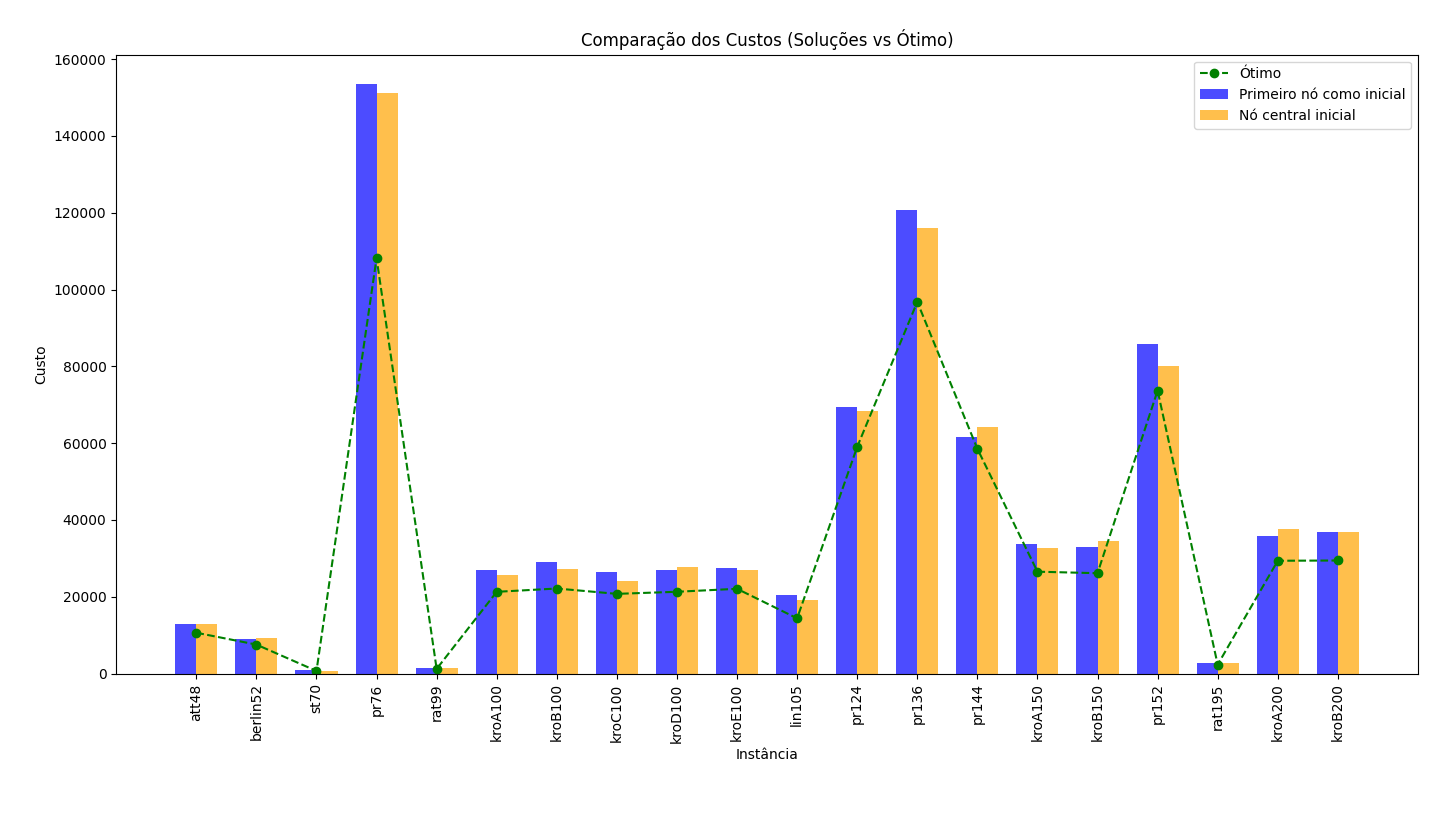
\includegraphics[width=1\linewidth]{graficos_custos.png}
    \caption{Resultados do custo do caminho das abordagens gulosas}
    \label{fig:Resultados abordagens gulosas}
\end{figure}

\begin{figure}[H]
    \centering
    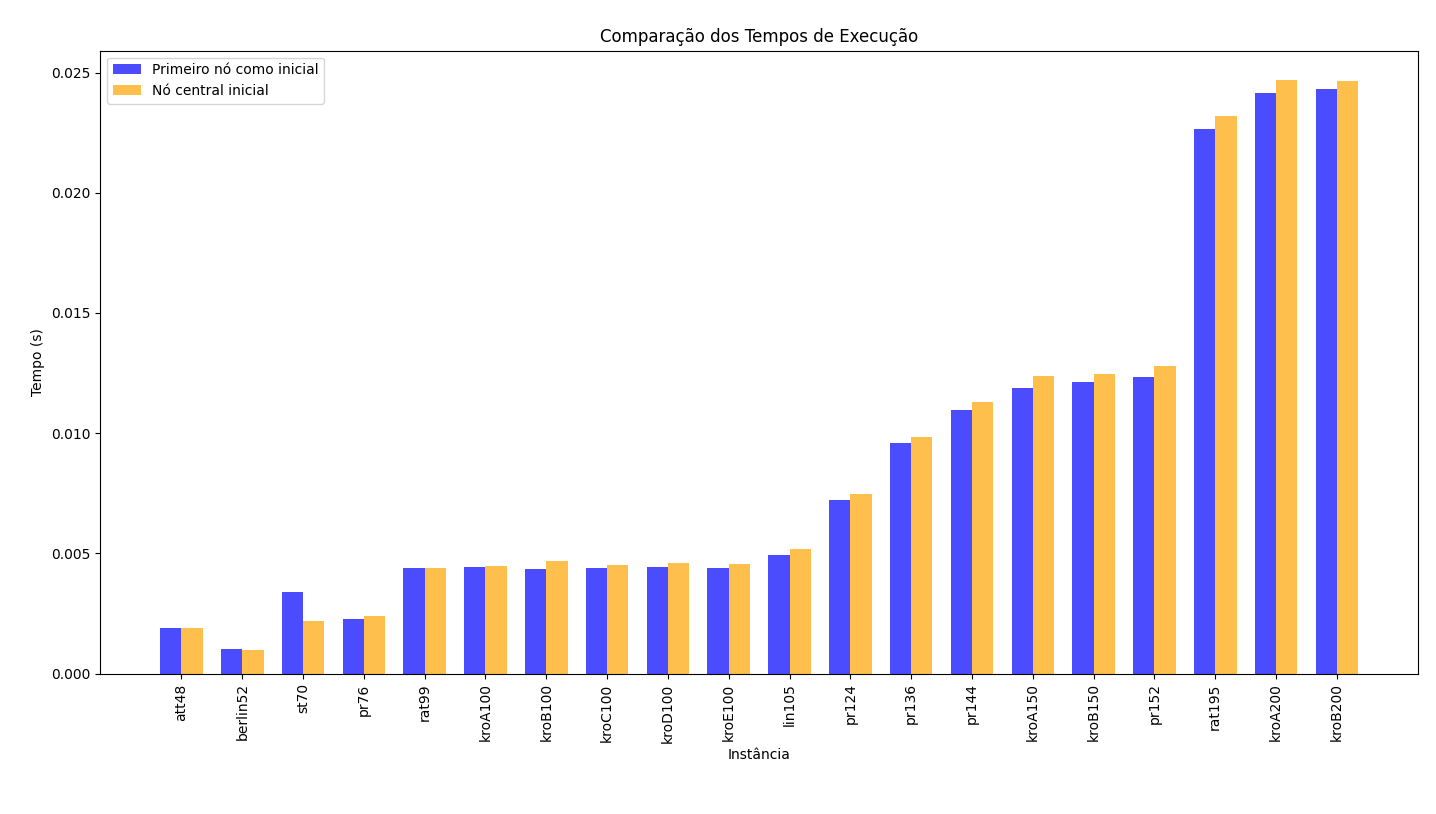
\includegraphics[width=1\linewidth]{graficos_tempo.png}
    \caption{Resultados do tempo gasto das abordagens gulosas}
    \label{fig:Resultados abordagens gulosas}
\end{figure}

Sumarizando a comparação dos resultados das diferentes abordagens, temos a tabela 1 que possui a melhor abordagem para cada uma das instâncias. Percebe-se que de maneira geral, a estratégia utilizando o nó central como inicio do caminho performou melhor. Mesmo que a abordagem com o primeiro nó como inicial possuindo vantagem em alguns dos casos maiores, a hipótese é que isso foi causado por propriedades de como as instâncias estão distribuídas, embora mais testes possam ser feitos para comprovar tal fato futuramente. 

\begin{table}[H]
\centering
\begin{tabular}{|c|p{12cm}|} \hline
\textbf{Heurística}               & \textbf{Instâncias onde obteve menor erro percentual}          \\ \hline
Primeiro nó como inicial & att48, berlin52, kroD100, pr144, kroB150, rat195, kroA200 \\ \hline
Nó central inicial       & st70, pr76, rat99, kroA100, kroB100, kroC100, kroE100, \newline lin105, pr107, pr124, pr136, kroA150, pr152, kroB200 \\ \hline
\end{tabular}
\caption{Comparação de abordagens - Instâncias com menor erro percentual}
\label{tab:comparison_reformatted}
\end{table}

Em todo caso, foi testado para uma instância adicional maior ambas as abordagens, em um problema envolvendo 3795 cidades, com os resultados mostrados abaixo nas tabelas 2 e 3. Percebe-se que mesmo para instâncias grandes em que o problema já se torna intratável (de maneira exata), as abordagens gulosas conseguem retornar resultados em tempo viável. Assim, em um primeiro momento, existe a ideía que escolher o nó central como inicial possui melhores resultados ao se extender o problema em maiores instâncias. Porém novamente, mais testes são necessários, além de otimizações na implementação para melhorar tanto o custo obtido quanto o tempo.

\begin{table}[H]
    \centering
    \begin{tabular}{|c|c|c|c|c|} \hline 
         \textbf{Instância} & \textbf{Ótimo} & \textbf{Custo} & \textbf{Tempo (s)} & \textbf{Erro Percentual (\%)} \\ \hline 
         fl3795       & 28772     & 36841.4    & 114.198  & 28.04 \\ \hline
    \end{tabular}
    \caption{Heurística gulosa - Primeiro nó como inicial}
    \label{tab:my_label}
\end{table}

\begin{table}[H]
    \centering
    \begin{tabular}{|c|c|c|c|c|} \hline 
         \textbf{Instância} & \textbf{Ótimo} & \textbf{Custo} & \textbf{Tempo (s)} & \textbf{Erro Percentual (\%)} \\ \hline 
         fl3795       & 28772     & 36145.5    & 106.698  & 25.62 \\ \hline
    \end{tabular}
    \caption{Heurística gulosa - Nó central como inicial}
    \label{tab:my_label}
\end{table}

\section{Referências}

\noindent \href{http://www.decom.ufop.br/prof/marcone/Disciplinas/InteligenciaComputacional/HeuristicasConstrutivas.pdf}{Slides sobre heurísticas construtivas e heurísticas gulosas}

\noindent \href{http://comopt.ifi.uni-heidelberg.de/software/TSPLIB95/}{Formato das instâncias de entrada e resultados ótimos}

\end{document}
